\documentclass{article}
\usepackage{tikz}
\usepackage{amsmath} % For math symbols like \mathcal, \theta
\usepackage{xcolor}
\usetikzlibrary{
    positioning,    % For relative node placement (right=of, etc.)
    arrows.meta,    % For arrow tip styles like Stealth
    shapes.geometric,% For shapes like rectangle and trapezium
    calc            % For coordinate calculations ($(...)!,! (...)$)
}

% Define a light blue color for the network fill
\definecolor{lightblue}{RGB}{210, 225, 240}

\begin{document}

\begin{figure}[htbp]
\centering
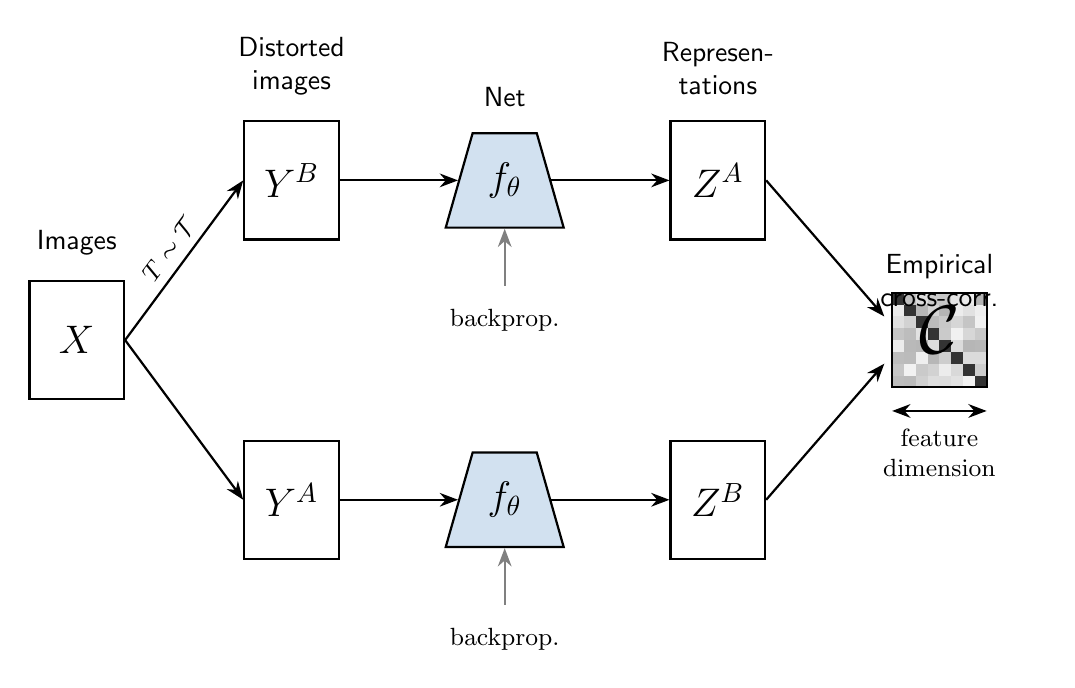
\begin{tikzpicture}[
    node distance=0.8cm and 1.5cm, % Vertical and horizontal spacing
    >=Stealth, % Default arrow tip style
    % Styles
    data_box/.style={ % Style for rectangular data/representation boxes
        rectangle,
        draw,
        thick,
        minimum width=1.2cm,
        minimum height=1.5cm,
        text centered,
        font=\Large % Larger font for math symbols
    },
    net_box/.style={ % Style for the trapezoidal network
        trapezium,
        trapezium angle=75, % Adjust angle for desired slant
        trapezium stretches=true, % Allows minimum width/height to work better
        draw,
        thick,
        fill=lightblue,
        minimum width=1.5cm,
        minimum height=1.2cm,
        text centered,
        font=\Large,
        inner xsep=0pt % Reduce horizontal padding if text is tight
    },
    arrow/.style={
        ->, thick
    },
    backprop_arrow/.style={
        <-, thick, gray % Backward arrow, gray color
    },
    label_text/.style={ % Style for descriptive labels
        font=\sffamily,
        text centered,
        align=center
    }
]

% --- Column 1: Input ---
\node[data_box] (X) {$X$};
\node[label_text, above=0.2cm of X] {Images};

% --- Column 2: Distorted Images ---
% Position Y nodes relative to X
\node[data_box] (YB) [above right=0.5cm and 1.5cm of X] {$Y^B$};
\node[data_box] (YA) [below right=0.5cm and 1.5cm of X] {$Y^A$};
% Column Label (centered vertically between Y nodes)
\node[label_text, above=0.2cm of YB] {Distorted\\images};
% Arrow from X splitting to Y's
\draw [arrow] (X.east) -- node[midway, above, sloped, font=\small] {$T \sim \mathcal{T}$} (YB.west);
\draw [arrow] (X.east) -- (YA.west);

% --- Column 3: Network ---
\node[net_box] (net1) [right=of YB] {$f_{\theta}$};
\node[net_box] (net2) [right=of YA] {$f_{\theta}$}; % Same network
% Column Label
\node[label_text, above=0.2cm of net1] {Net};
% Arrows into network
\draw [arrow] (YB.east) -- (net1.west);
\draw [arrow] (YA.east) -- (net2.west);
% Backprop arrows and labels
\node (bp1) [below=0.6cm of net1] {}; % Helper node for arrow start
\node (bp2) [below=0.6cm of net2] {}; % Helper node for arrow start
\draw [backprop_arrow] (net1.south) -- (bp1.center);
\draw [backprop_arrow] (net2.south) -- (bp2.center);
\node [label_text, font=\small, below=0.05cm of bp1] {backprop.};
\node [label_text, font=\small, below=0.05cm of bp2] {backprop.};


% --- Column 4: Representations ---
\node[data_box] (ZA) [right=of net1] {$Z^A$};
\node[data_box] (ZB) [right=of net2] {$Z^B$};
% Column Label
\node[label_text, above=0.2cm of ZA] {Represen-\\tations};
% Arrows into representations
\draw [arrow] (net1.east) -- (ZA.west);
\draw [arrow] (net2.east) -- (ZB.west);

% --- Column 5: Correlation Matrix ---
% Calculate center position for the matrix - Reduced horizontal offset
\coordinate (matrix_center) at ($(ZA.east)!0.5!(ZB.east) + (2.2cm, 0)$);
% Matrix parameters - Adjusted size
\def\matrixsize{1.2cm} % Match data_box width
\def\N{8} % Number of cells per side (NxN matrix)
% Define \celldim as a dimension and calculate its value
\newdimen\celldim
\pgfmathsetlength{\celldim}{\matrixsize/\N} % Calculate the dimension

% Draw the matrix using nested loops
\begin{scope}[shift={(matrix_center)}, xshift=-0.5*\matrixsize, yshift=0.5*\matrixsize] % Shift origin to top-left corner
    \foreach \i in {1,...,\N} { % Row index
        \foreach \j in {1,...,\N} { % Column index

            % --- Start Refined Calculation ---
            % Calculate numerical multipliers first
            \pgfmathtruncatemacro{\xmultiplier}{\j-1} % Integer multiplier for x
            \pgfmathtruncatemacro{\ymultiplier}{-\i}  % Integer multiplier for y

            % Define the coordinate using the multipliers and the dimension
            \coordinate (cellpos) at (\xmultiplier*\celldim, \ymultiplier*\celldim);
            % --- End Refined Calculation ---

            % Determine color string (same logic as before)
            \pgfmathparse{(\i == \j) ? 0 : 1}
            \ifdim\pgfmathresult pt=0pt
                \edef\cellfillcolor{black!80}
            \else
                \pgfmathsetmacro{\randompercent}{rnd*50+10}
                \edef\cellfillcolor{gray!\randompercent}
            \fi

            % Draw the filled cell using the dimension \celldim
            % The rectangle command is robust with dimensions
            \fill[\cellfillcolor] (cellpos) rectangle ++(\celldim, \celldim);
        }
    }
    % Draw border around the matrix
    \draw[thick] (0,0) rectangle (\matrixsize, -\matrixsize); % Border uses \matrixsize
    % Add feature dimension label below
    \draw[<->, thick] (0, -\matrixsize - 0.3cm) -- node[below=0.1cm, label_text, font=\small] {feature\\dimension} (\matrixsize, -\matrixsize - 0.3cm);
\end{scope} % End of matrix scope

% Column Label and Math Symbol for Matrix
\node[label_text, text width=2.5cm, above=0.3cm of matrix_center] {Empirical\\cross-corr.};
\node[font=\Huge, above=0.0cm of matrix_center, yshift=-0.3cm] {$\mathcal{C}$};

% Arrows from Representations to Matrix
% Endpoints adjust automatically based on matrix_center and matrixsize
\draw [arrow] (ZA.east) -- ($(matrix_center)+(-0.5*\matrixsize-0.1cm, 0.25*\matrixsize)$);
\draw [arrow] (ZB.east) -- ($(matrix_center)+(-0.5*\matrixsize-0.1cm, -0.25*\matrixsize)$);


\end{tikzpicture}
\caption{Illustration of the Barlow Twins method (or similar self-supervised approach) showing image augmentation, encoding, representation extraction, and cross-correlation matrix computation.}
\label{fig:ssl_crosscorr}
\end{figure}

\end{document}